\documentclass[11pt,a4paper]{article}

% ── Packages ──
\usepackage[margin=0.9in]{geometry}
\usepackage{amsmath,amssymb,amsthm}
\usepackage{booktabs}
\usepackage{graphicx}
\usepackage[dvipsnames]{xcolor}
\usepackage{hyperref}
\usepackage{pgfplots}
\usepackage{siunitx}
\usepackage{caption}
\usepackage{float}
\usepackage{fancyhdr}
\usepackage{microtype}
\usepackage{tabularx}
\usepackage{multirow}

\pgfplotsset{compat=1.18}
\sisetup{group-separator={,}, group-minimum-digits=4}

\hypersetup{
  colorlinks=true,
  linkcolor=MidnightBlue,
  citecolor=MidnightBlue,
  urlcolor=MidnightBlue
}

\pagestyle{fancy}
\fancyhf{}
\fancyhead[L]{\small\textsc{ANDES Optimization Report}}
\fancyhead[R]{\small\thepage}
\renewcommand{\headrulewidth}{0.4pt}

% ── Title ──
\title{%
  \vspace{-1cm}
  \textbf{Optimizing ANDES:}\\[4pt]
  \Large From 12 Hours to 23 Seconds on the\\
  GO BP 12.4M-Pair Self-vs-Self Benchmark%
}
\author{Charlie Cruz}
\date{}

\begin{document}
\maketitle
\thispagestyle{fancy}

% ══════════════════════════════════════════════════════════════════════════════
\begin{abstract}
	\noindent
	ANDES computes gene-set similarity in embedding spaces using a reciprocal
	Best Match Average (BMA) score normalized by a Monte Carlo null distribution.
	The original implementation required \num{43520} seconds (roughly 12.1 hours)
	to score 3{,}518 Gene Ontology Biological Process terms against themselves,
	corresponding to 12.4~million term pairs using 32 workers on a shared-memory
	server.

	We describe four complementary optimizations: batched vectorized sampling
	with a shared size-pair null cache, prefix-coupled null construction, exact
	gene-to-term best-match query scoring, and symmetric matrix reuse. Together,
	these reduce the GO~BP self-vs-self benchmark to 23.2~seconds, a
		1{,}876$\times$ end-to-end speedup.

	The optimized query scorers preserve the published BMA and ranked enrichment
	score definitions exactly up to floating-point precision. For BMA validation,
	the optimized true scores match direct pairwise scoring with Pearson
	$r = 1.000$ and max $|\Delta| = 2.7 \times 10^{-7}$. The optimized null
	builder preserves the marginal null distribution for each size pair, yielding
	statistically equivalent z-score rankings rather than bitwise identical
	z-scores (Spearman $\rho = 0.9995$; top-500 overlap 99.6\%).
	Ranked ANDES is reduced from 652~seconds to 16.4~seconds on the GSE3467
	benchmark. All optimizations are exposed as configurable modes in the ANDES
	codebase.
\end{abstract}

\vspace{0.8em}
\hrule
\vspace{1.2em}

% ══════════════════════════════════════════════════════════════════════════════
\section{Introduction}

ANDES~\cite{li2024andes} computes gene set similarity by embedding genes into
a vector space learned from a consensus protein-protein interaction network
using node2vec, then measuring Best Match Average (BMA) similarity between
gene sets. For a pair of gene sets $X_i$ and $Y_j$ with L2-normalized
embedding rows $E$ and cosine similarity
$\mathrm{sim}(a,b) = E_a \cdot E_b$, the BMA score is:

\begin{equation}
	\label{eq:bma}
	\mathrm{BMA}(X_i, Y_j) \;=\;
	\frac{%
		\displaystyle\sum_{x \in X_i} \max_{y \in Y_j} \mathrm{sim}(x,y)
		\;+\;
		\displaystyle\sum_{y \in Y_j} \max_{x \in X_i} \mathrm{sim}(x,y)
	}{|X_i| + |Y_j|}
\end{equation}

Each true score is normalized to a z-score against a null distribution
estimated by Monte Carlo: for each unique size pair $(m,k)$, random gene sets
of size $m$ and $k$ are drawn from the background population and scored
$N_\text{iter}$ times to estimate $(\mu_{m,k}, \sigma_{m,k})$.

The original implementation (Section~\ref{sec:baseline}) evaluates
Equation~\ref{eq:bma} independently for every term pair and estimates an
independent null distribution for every pair as well. On the Gene Ontology
Biological Process benchmark (3{,}518 terms, 20{,}363-gene embedding, sizes
10--300), this required approximately 12~hours of wall-clock time.

The central observation behind the work reported here is that ANDES repeatedly
recomputes quantities that depend only on gene-set size or target-term
identity, not on which specific source term is being scored. The null
distribution depends on $(m,k)$, not on term names; the directed best match
from a gene to a target term can be reused across all source terms. The
optimized implementation exploits these two invariances, together with
prefix-coupled Monte Carlo sampling and symmetric-matrix folding, to reduce
total wall-clock time to 23.2~seconds while preserving the mathematical
identity of the BMA statistic and the marginal validity of the null
distribution for each size pair.

A key distinction runs through the report: true-score equality between
the original and optimized scorers is algebraic (the BMA factorization is
exact), while z-score equality is statistical (the null estimator changed
from per-pair independent Monte Carlo to a shared prefix-coupled cache with
\texttt{ddof=1} and float32 arithmetic). The target for z-scores is therefore
stability of biological rankings, not bitwise reproduction.

% ══════════════════════════════════════════════════════════════════════════════
\section{Benchmark Environment}

All benchmarks were run on \texttt{mochi.cs.rice.edu}, a shared-memory Dell
PowerEdge server with Intel Xeon Gold 5220 processors (144 logical cores at
up to 3.9\,GHz) and 772\,GB of RAM, running Red Hat Enterprise Linux 8.10
(kernel 4.18.0). The software stack used CPython 3.11.15 with NumPy 1.26.4
(linked against OpenBLAS 0.3.23 with AVX-512 support), SciPy 1.12.0, and
Numba 0.59.1. Per-process BLAS thread counts were pinned to 1
(\texttt{OMP\_NUM\_THREADS=1}, \texttt{MKL\_NUM\_THREADS=1},
\texttt{OPENBLAS\_NUM\_THREADS=1}) so that parallelism is managed explicitly
through Python \texttt{multiprocessing} and \texttt{ThreadPoolExecutor}
workers.

The dataset is held constant across all benchmarks: a node2vec consensus PPI
embedding of 20{,}363 genes in 128 dimensions, scored against the GO
Biological Process database filtered to 3{,}518 terms with sizes
$10 \le |X| \le 300$. The background population consists of 9{,}247 genes
appearing in both the embedding and the gene set database. All runs use
	1{,}000 Monte Carlo iterations with random seed 12345. The full self-vs-self
job produces $3{,}518^2 = 12{,}376{,}324$ scored pairs (6{,}189{,}921 unique
after symmetric folding) across 62{,}001 unique size pairs $(m,k)$.

All reported times include null cache construction from scratch (cold cache).
Output CSV writing is excluded except where noted. The standard ANDES mode
(\texttt{distinct=False}) is used throughout; the size-pair null cache and
best-match factorization assume no dynamic per-pair overlap removal.

% ══════════════════════════════════════════════════════════════════════════════
\section{Original Implementation (Baseline)}
\label{sec:baseline}

The original ANDES implementation (\texttt{old\_andes.py},
\texttt{set\_analysis\_func.py}) first computes the full $N \times N$ cosine
similarity matrix $S$ via sklearn's \texttt{cosine\_similarity}. The
embedding is loaded through \texttt{np.loadtxt}, which returns float64 by
default; the sklearn cosine matrix is therefore computed in float64. The
script then dispatches each of the 12.4~million term pairs $(X_i, Y_j)$ as
a separate \texttt{multiprocessing.Pool} task. Each task slices $S[X_i,Y_j]$
to get the pairwise similarity sub-matrix, computes
$\mathrm{BMA}(X_i, Y_j)$ via row-max and column-max, draws $N_\text{iter}$
random gene sets of sizes $|X_i|$ and $|Y_j|$ using \texttt{random.sample},
and computes a null BMA for each to return $z = (\text{true} - \mu) / \sigma$
(using \texttt{np.std} with NumPy's default \texttt{ddof=0}).

This design has three critical bottlenecks. First, each of the 12.4~million
term pairs estimates its own null from scratch; pairs with the same sizes
$(m,k)$ redundantly re-estimate the same distribution. Second,
random sampling occurs inside the innermost Monte Carlo loop, creating heavy
Python-level overhead across billions of calls. Third, the full similarity
matrix must be materialized in memory (over 3\,GB in float64 for
$N = 20{,}363$), and each BMA evaluation extracts a sub-matrix via
Python-level fancy indexing.

On Mochi with 32 workers, total wall-clock time was \num{43520}\,s, of which
\num{43502}\,s was the scoring loop. The $S$-matrix construction accounted for
only 2.1\,s; runtime is completely dominated by per-pair Monte Carlo null
estimation.

% ══════════════════════════════════════════════════════════════════════════════
\section{Optimization 1: Batched Vectorized Scoring with Shared Null Cache}

The first optimization replaces the per-pair Monte Carlo loop with a shared
null cache and introduces several vectorization techniques. These are a mix of
statistical reuse (one cache entry per size pair rather than per term pair)
and engineering improvements (Numba kernels, batched BLAS, cost-balanced
chunking).

\paragraph{Shared null cache.}
The null distribution depends only on the size pair $(m,k)$, not on which
specific terms are involved. A shared \texttt{NullCacheBMA} stores one
$(\mu, \sigma)$ per unique $(m,k)$, reducing the number of independent Monte
Carlo estimations from 12.4~million to 62{,}001 unique size pairs.

\paragraph{Batched Fisher-Yates sampling.}
Python's \texttt{random.sample} is not necessarily $O(N)$ for small samples
from a sequence, but calling it repeatedly inside the innermost Monte Carlo
loop still incurs substantial interpreter overhead. The optimized path
removes most of that overhead: swap indices for $b$ samples are generated in
a single \texttt{rng.integers} call, and a compiled partial Fisher-Yates
kernel applies the swaps at $O(b \cdot m)$ cost.

\paragraph{Batched GEMM for null estimation.}
Rather than computing BMA one iteration at a time, $b$ random gene sets are
packed into tensors of shape $(b, m, d)$ and $(b, k, d)$. A single
\texttt{np.matmul} call produces the $(b, m, k)$ similarity tensor;
vectorized \texttt{max} and \texttt{sum} extract all $b$ BMA scores
simultaneously, amortizing BLAS launch overhead.

\paragraph{Cost-balanced parallel chunking.}
Size pairs are sorted by descending cost ($m \times k$) and distributed to
worker chunks with a greedy load-balancing heuristic, preventing any single
worker from accumulating all the expensive large-size pairs.

\paragraph{Batched row query scorer.}
For the query stage, all gene-set-2 embedding blocks are concatenated into a
single $(T_2, d)$ matrix where $T_2 = \sum_j |Y_j|$. For each gene-set-1
term $X_i$ of size $m$, a single GEMM produces $(m, T_2)$;
\texttt{np.maximum.reduceat} then extracts per-term row-maxima without
looping over individual terms.

\paragraph{Result.}
On Mochi with 32 workers, total time drops to 436.4\,s (cache build 391.6\,s,
query scoring 34.2\,s), a $100\times$ speedup over the original.
With 8 workers, the same configuration takes 1{,}504.6\,s (cache 1{,}444.8\,s,
query 57.6\,s). The pairwise null build scales reasonably with worker count
but remains the dominant bottleneck: 62{,}001 size pairs
$\times$ 1{,}000 iterations still amounts to 62~million independent BMA
simulations.

% ══════════════════════════════════════════════════════════════════════════════
\section{Optimization 2: Prefix-Coupled Null Construction}

The pairwise null builder performs $62{,}001 \times 1{,}000 = 62{,}001{,}000$
independent Monte Carlo BMA evaluations. The prefix-coupled builder replaces
this with just 1{,}000 iterations, each computing a single
$(\max_m \times \max_k)$ similarity matrix from random permutation prefixes
and extracting all requested size pairs via cumulative operations.

\subsection{Why prefixes are valid random sets}
\label{sec:prefix-proof}

The theoretical basis is a standard result in combinatorics. Let $P$ be a
background population of size $N$, and let $\pi$ be a permutation of $P$
drawn uniformly at random from all $N!$ orderings. For any fixed $m$, the
unordered set $\{\pi_1, \ldots, \pi_m\}$ is uniformly distributed over all
$\binom{N}{m}$ subsets of size $m$. The reason is that every particular
$m$-element subset $S$ appears as the first $m$ elements in exactly
$m!\,(N-m)!$ permutations (any ordering of $S$ in the first $m$ positions,
times any ordering of the complement in the remaining positions), so:

\[
	\Pr\bigl(\{\pi_1, \ldots, \pi_m\} = S\bigr)
	= \frac{m!\,(N-m)!}{N!}
	= \frac{1}{\binom{N}{m}}
\]

This means using the first $m$ elements of a random permutation as a null
sample is statistically identical to drawing $m$ elements uniformly without
replacement. The prefix does not bias the null for any single size $m$.

\subsection{One matrix contains all prefix-pair BMA scores}

Each Monte Carlo iteration samples two independent full-length random permutations
$\pi_1$ and $\pi_2$ of the two background populations and takes prefixes
$X = E[\pi_1[:\max_m]]$ and $Y = E[\pi_2[:\max_k]]$.
The iteration then computes:

\[
	A = X \, Y^\top \quad\in\;\mathbb{R}^{\max_m \times \max_k}
\]

For any requested prefix pair $(m, k)$ with $m \le \max_m$ and $k \le \max_k$,
the upper-left $m \times k$ submatrix $A[{:}m,\, {:}k]$ is exactly the
similarity matrix that would have been computed for independently drawn
random sets of sizes $m$ and $k$. Cumulative maxima recover the BMA
components for every such upper-left rectangle:

\begin{align}
	\text{row\_best}[i, j]
	 & = \max_{j' \le j}\, A[i, j']
	\notag                                                                                                        \\
	\text{col\_best}[i, j]
	 & = \max_{i' \le i}\, A[i', j]
	\notag                                                                                                        \\[4pt]
	\text{row\_sum}[m, k]
	 & = \textstyle\sum_{i=1}^{m} \text{row\_best}[i, k]
	 &                                                               & \text{(directed sum, source $\to$ target)}
	\notag                                                                                                        \\
	\text{col\_sum}[m, k]
	 & = \textstyle\sum_{j=1}^{k} \text{col\_best}[m, j]
	 &                                                               & \text{(directed sum, target $\to$ source)}
	\notag                                                                                                        \\[4pt]
	\text{score}[m, k]
	 & = \frac{\text{row\_sum}[m, k] + \text{col\_sum}[m, k]}{m + k}
	 &                                                               & \text{(BMA for prefix $(m,k)$)}
\end{align}

The cumulative sums and maxima (\texttt{np.cumsum}, \texttt{np.maximum.accumulate})
are computed once on the $\max_m \times \max_k$ grid. Running Welford
accumulators are then updated for each requested $(m,k)$. This is not
approximating BMA; it is reusing one larger sampled matrix to evaluate many
exact prefix BMA scores.

\subsection{Complexity reduction}

The speedup comes from replacing the sum over all requested rectangles with
one maximal rectangle per iteration:

\[
	\underbrace{O\!\bigl(N_\text{iter} \cdot \textstyle\sum_{(m,k)} m \cdot k \cdot d\bigr)}_{\text{pairwise: 62M BMA evaluations}}
	\;\;\longrightarrow\;\;
	\underbrace{O\!\bigl(N_\text{iter} \cdot \max_m \cdot \max_k \cdot d\bigr)
		+ O\!\bigl(N_\text{iter} \cdot \max_m \cdot \max_k\bigr)
		+ O\!\bigl(N_\text{iter} \cdot |\mathcal{U}|\bigr)}_{\text{prefix: 1{,}000 matrix ops + cumulative extraction + cache updates}}
\]

For the GO~BP benchmark with $\max_m = \max_k = 300$, $d = 128$, and 62{,}001
requested size pairs, a single $300 \times 300$ matrix per iteration replaces
the summed work of all 62{,}001 independent estimations.

\subsection{Correlation changes; marginal nulls do not}

This is the important caveat. In the old pairwise builder, null samples for
different size pairs are independent because each $(m,k)$ is simulated
separately. In the prefix-coupled builder, null samples for different size
pairs share the same random permutations, so neighboring $(m,k)$ estimates
are statistically correlated. However, for any fixed $(m,k)$, the sampled
prefix sets have exactly the same distribution as independently drawn random
sets without replacement (Section~\ref{sec:prefix-proof}). Since ANDES uses only the marginal
mean and standard deviation for the observed size pair:

\[
	z_{ij} = \frac{\mathrm{BMA}_\text{true}(X_i, Y_j) - \mu_{m,k}}{\sigma_{m,k}}
\]

this correlation across cache entries does not bias any individual z-score.
It only changes the joint Monte Carlo noise structure across sizes, which
ANDES does not depend on.

\paragraph{Result.}
Comparing apples-to-apples at 8 workers, cache build drops from 1{,}444.8\,s
(pairwise) to 2.5\,s (prefix); roughly a $580\times$ improvement in null
construction. Query scoring remains 58.7\,s (identical scorer), giving a
total of 62.7\,s. Cumulative speedup from baseline: $694\times$.

% ══════════════════════════════════════════════════════════════════════════════
\section{Optimization 3: Exact Gene-to-Term Best-Match Scoring}

With the null cache bottleneck removed, the query scorer (58.7\,s) becomes
dominant. The batched row scorer computes, for each source term $X_i$, a full
GEMM against the concatenated target blocks. For $N_1 = N_2 = 3{,}518$ terms,
this means 3{,}518 GEMM calls, each producing an $(m_i, T_2)$ matrix. Many
source terms share the same genes, so the same gene-to-target-term best-match
values are recomputed redundantly across rows.

The best-match scorer eliminates this redundancy by precomputing the reusable
directed best-match matrix:

\[
	B_2[g, j] = \max_{y \in Y_j} \mathrm{sim}(g, y) \quad
	\text{for all genes } g \text{ and target terms } Y_j
\]

Let $M_1$ be the sparse term-by-gene membership matrix for database~1, where
$M_1[i,g] = 1$ if gene $g \in X_i$ and 0 otherwise. Then the directed score
from every source term to every target term is a single sparse-times-dense
multiplication:

\begin{align}
	D_{12}[i,j]
	 & = \sum_g M_1[i,g] \;\cdot\; B_2[g,j] \notag           \\
	 & = \sum_{x \in X_i} \max_{y \in Y_j} \mathrm{sim}(x,y)
	\label{eq:d12-proof}
\end{align}

Equation~\ref{eq:d12-proof} shows that $D_{12} = M_1 \, B_2$ computes
exactly the directed half of BMA (the first sum in Equation~\ref{eq:bma}).
The reverse direction is symmetric: $B_1[g, i] = \max_{x \in X_i}
	\mathrm{sim}(g, x)$ and $D_{21} = M_2 \, B_1$, recovering the second sum.
The exact ANDES true-score matrix is:

\begin{equation}
	\label{eq:bestmatch}
	\mathrm{BMA}[i,j] = \frac{D_{12}[i,j] + D_{21}^\top[i,j]}{|X_i| + |Y_j|}
\end{equation}

This is algebraically identical to Equation~\ref{eq:bma}; the gain is
purely computational. Each gene-to-term best-match value is computed once and
reused across all source terms:

\[
	\underbrace{O\!\bigl(d \cdot \textstyle\sum_i |X_i| \cdot
		\textstyle\sum_j |Y_j|\bigr)}_{\text{batched row scorer}}
	\;\;\longrightarrow\;\;
	\underbrace{O\!\bigl(d \cdot N_\text{genes} \cdot
		\textstyle\sum_j |Y_j|\bigr)}_{\text{build }B_2}
	+
	\underbrace{O\!\bigl(N_2 \cdot \textstyle\sum_i |X_i|\bigr)}_{\text{sparse-times-dense aggregation}}
\]

On the GO~BP benchmark, a full float32 $B[g,t]$ matrix occupies approximately
$20{,}363 \times 3{,}518 \times 4 \approx 286$\,MB. Larger databases are
handled by term chunking, controlled by \texttt{--query-memory-mb}.

\paragraph{Result.}
Query scoring drops from 58.7\,s to 36.4\,s. Total time: 40.4\,s (including
cache build of 2.4\,s).

% ══════════════════════════════════════════════════════════════════════════════
\section{Optimization 4: Symmetric Matrix Reuse}

For self-vs-self comparisons (geneset1 $=$ geneset2), the two gene-set
databases are identical, which means $B_1 = B_2 = B$ and $M_1 = M_2 = M$.
The directed score matrices are therefore also identical:

\[
	D_{12} = D_{21} = M\,B
\]

and the full BMA matrix simplifies to:

\[
	\mathrm{BMA}[i,j] = \frac{D[i,j] + D[j,i]}{|X_i| + |X_j|}
\]

The computational gain is avoiding the second directed best-match matrix
construction entirely. Instead of building $B_1$ and $B_2$ separately (each
requiring a full $N_\text{genes} \times N_\text{terms}$ GEMM pass), the
scorer builds $B$ once and obtains the full symmetric score via
$D + D^\top$. The output matrix still has $N^2$ entries. Mathematically,
only $\binom{N}{2} + N = 6{,}189{,}921$ unique scores exist because
$\mathrm{BMA}[i,j] = \mathrm{BMA}[j,i]$, but the main runtime savings come
from reusing the single directed best-match matrix.

This symmetry statement is about the true BMA score. In self-vs-self mode,
the null distribution for $(m,k)$ is the same as for $(k,m)$, but a Monte
Carlo cache keyed by ordered pairs can store slightly different estimates for
the two orientations. Canonicalizing size-pair keys as
$(\min(m,k), \max(m,k))$ would enforce z-score symmetry; otherwise the true
scores remain symmetric while transposed z-scores may differ by Monte Carlo
noise.

\paragraph{Result.}
Query scoring: 18.0\,s. Total: 23.2\,s. Cumulative speedup from
baseline: $1{,}876\times$.

\paragraph{Worker scaling.}
Running the same configuration with 32 workers yields 24.3\,s (query 18.7\,s),
confirming that the remaining bottleneck is memory bandwidth and GEMM
throughput, not parallelism.

% ══════════════════════════════════════════════════════════════════════════════
\section{Summary of the Optimization Cascade}

Table~\ref{tab:headline} collects all benchmarked configurations.
Figure~\ref{fig:cascade} shows the progression on a log scale.

\begin{table}[H]
	\centering
	\caption[End-to-end wall-clock times for the GO BP self-vs-self benchmark]{End-to-end wall-clock times for the GO BP self-vs-self benchmark
			(3{,}518 terms, 12.4M pairs, 1{,}000 Monte Carlo iterations).
		All times from JSON benchmark reports; ``w'' denotes worker count.}
	\label{tab:headline}
	\vspace{-0.4em}
	\begin{tabularx}{\textwidth}{@{}Xcrrrr@{}}
		\toprule
		Configuration & Workers & Total (s)   & Cache (s)  & Query (s)   & Speedup         \\
		\midrule
		Original ANDES
		              & 32      & \num{43520} & ---        & \num{43502} & $1\times$       \\
		Batched + pairwise null
		              & 32      & 436.4       & 391.6      & 34.2        & $100\times$     \\
		Batched + pairwise null
		              & 8       & \num{1505}  & \num{1445} & 57.6        & $29\times$      \\
		Batched + prefix null
		              & 8       & 62.7        & 2.5        & 58.7        & $694\times$     \\
		Bestmatch + prefix
		              & 8       & 40.4        & 2.4        & 36.4        & $1{,}077\times$ \\
		Bestmatch + prefix + symmetric
		              & 8       & 23.2        & 3.0        & 18.0        & $1{,}876\times$ \\
		Bestmatch + prefix + symmetric
		              & 32      & 24.3        & 3.1        & 18.7        & $1{,}791\times$ \\
		\bottomrule
	\end{tabularx}
\end{table}

\begin{figure}[H]
	\centering
	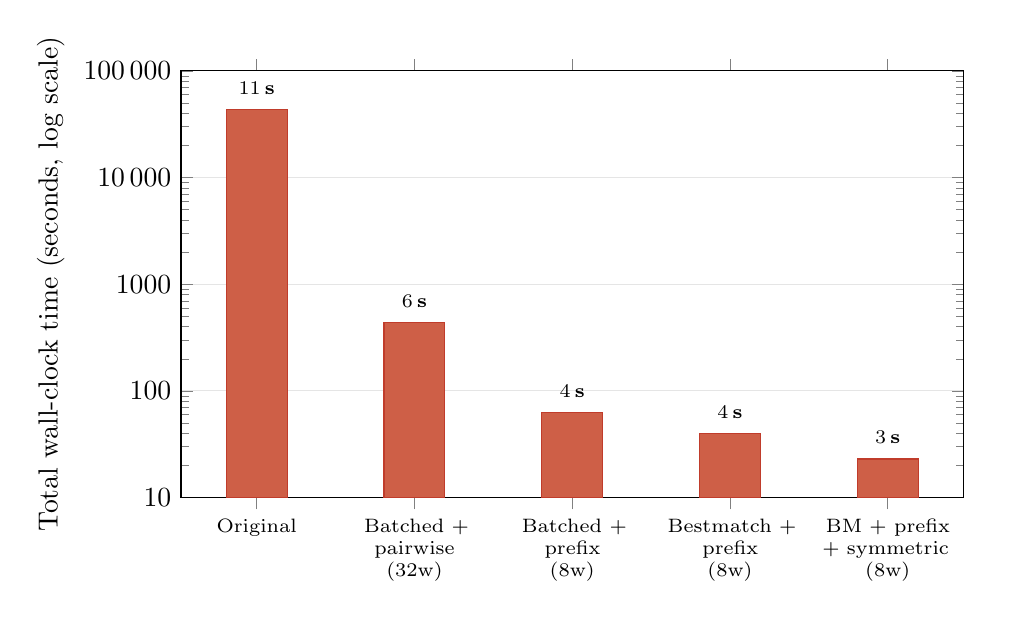
\begin{tikzpicture}
		\begin{axis}[
				ybar,
				bar width=22pt,
				width=0.95\textwidth,
				height=7cm,
				ymode=log,
				log origin=infty,
				ylabel={Total wall-clock time (seconds, log scale)},
				ymin=10,
				ymax=100000,
				ytick={10,100,1000,10000,100000},
				yticklabels={10,100,\num{1000},\num{10000},\num{100000}},
				xtick=data,
				symbolic x coords={Original,{Batched +\\pairwise\\(32w)},{Batched +\\prefix\\(8w)},{Bestmatch +\\prefix\\(8w)},{BM + prefix\\+ symmetric\\(8w)}},
				x tick label style={align=center, font=\scriptsize, text width=2.4cm},
				nodes near coords={\pgfmathprintnumber[precision=0]{\pgfplotspointmeta}\,s},
				nodes near coords style={font=\scriptsize\bfseries, above, yshift=2pt},
				every node near coord/.append style={text=black},
				enlarge x limits=0.12,
				ymajorgrids=true,
				grid style={gray!20},
				xmajorgrids=false,
			]
			\addplot[fill=BrickRed!65, draw=BrickRed!85] coordinates {
					(Original, 43520)
					({Batched +\\pairwise\\(32w)}, 436)
					({Batched +\\prefix\\(8w)}, 63)
					({Bestmatch +\\prefix\\(8w)}, 40)
					({BM + prefix\\+ symmetric\\(8w)}, 23)
				};
		\end{axis}
	\end{tikzpicture}
	\caption{Wall-clock time at each optimization stage (log scale). Each bar
		represents cumulative application of all optimizations up to that point.}
	\label{fig:cascade}
\end{figure}

The cascade shows that the speedup is not due to one isolated low-level
optimization. The first batched implementation removes Python overhead and
per-pair query inefficiency, but the null cache remains expensive when each
size pair is simulated independently. Prefix-coupled null construction removes
that bottleneck entirely, shifting runtime to true-score query evaluation.
The gene-to-term best-match formulation then attacks the new bottleneck by
reusing directed best-match values across all source terms, and symmetric
reuse halves the dominant best-match construction work in self-vs-self runs.

Table~\ref{tab:breakdown} provides a finer-grained timing breakdown. The
shift in bottleneck is visible: in the original, the per-pair scoring loop
dominates; after the batched rewrite, the pairwise null cache dominates;
after the prefix null, the query scorer dominates; after bestmatch +
symmetric reuse, no single stage dominates and the remaining time is split
between cache construction and query scoring.

\begin{table}[H]
	\centering
	\caption{Stage-by-stage timing breakdown (seconds). The original ``scoring''
		stage includes null estimation; the optimized pipeline separates these.
		Dashes indicate stages not separately instrumented in that configuration.}
	\label{tab:breakdown}
	\smallskip
	\small
	\setlength{\tabcolsep}{5pt}
	\begin{tabular}{@{}lrrrrr@{}}
		\toprule
		Stage                        & Original                  & \shortstack{Batch+PW\\(32w)} &
		\shortstack{Batch+Pfx\\(8w)} & \shortstack{BM+Pfx\\(8w)} &
		\shortstack{BM+Pfx+Sym\\(8w)}                                                                                 \\
		\midrule
		Load                         & 0.7                       & 0.7                          & 0.7   & ---  & 0.9  \\
		$S$-matrix / norm            & 2.1                       & 0.008                        & 0.008 & ---  & 0.01 \\
		Gene sets                    & 0.3                       & 0.4                          & 0.3   & ---  & 0.5  \\
		Numba warmup                 & ---                       & 0.9                          & 0.4   & ---  & 0.7  \\
		Term blocks                  & ---                       & 0.1                          & 0.1   & ---  & 0.1  \\
		Cache build                  & ---                       & 391.6                        & 2.5   & 2.4  & 3.0  \\
		Query scoring                & \num{43502}               & 34.2                         & 58.7  & 36.4 & 18.0 \\
		\midrule
		Total                        & \num{43520}               & 436.4                        & 62.7  & 40.4 & 23.2 \\
		\bottomrule
	\end{tabular}
\end{table}

% ══════════════════════════════════════════════════════════════════════════════
\section{Optimization Taxonomy}

It is worth distinguishing the algorithmic contributions from the engineering
ones, since the two categories compound but are conceptually different.

\begin{table}[H]
	\centering
	\caption{Classification of optimizations by type.}
	\smallskip
	\small
	\begin{tabularx}{\textwidth}{@{}lX@{}}
		\toprule
		Type                  & Optimization                                              \\
		\midrule
		Statistical reuse     & One null cache entry per $(m,k)$ instead of per term pair \\[2pt]
		Null algorithm        & Prefix-coupled null construction via cummax/cumsum on a
		single $(\max_m \times \max_k)$ matrix per iteration                              \\[2pt]
		Query algorithm       & Gene-to-term best-match matrix $B[g,t]$ with sparse
		$M \cdot B$ aggregation                                                           \\[2pt]
		Symmetry exploitation & Self-vs-self: build $B$ once, combine via
		$D + D^\top$                                                                      \\[2pt]
		Engineering           & Batched GEMM, Numba partial Fisher-Yates, Welford online
		accumulators, cost-balanced parallel chunking, term-block precomputation          \\
		\bottomrule
	\end{tabularx}
\end{table}

The gene-to-term best-match matrix and the prefix-coupled null construction
are real algorithmic changes to how ANDES computes; the rest are
vectorization and systems-level improvements that make the same algorithm
faster on modern hardware.

% ══════════════════════════════════════════════════════════════════════════════
\section{Ranked ANDES (Embedding-Based GSEA)}

ANDES also supports a ranked enrichment mode. For a ranked gene list $R$ of
length $L$ and a gene set $X_t$, the enrichment score is the maximum signed
cumulative sum of centered column-maxima:

\begin{align*}
	S[r, t]        & = \max_{x \in X_t} \mathrm{sim}(R_r, x) \\
	\mathrm{ES}[t] & =
	\mathrm{running}\!\left[\arg\max_r |\mathrm{running}[r,t]|\right]
	\;,\quad
	\mathrm{running}[:,t] = \mathrm{cumsum}\bigl(S[:,t] - \overline{S[:,t]}\bigr)
\end{align*}

That is, the enrichment score is the signed value of the running centered
sum at the rank where its absolute deviation from zero is largest.

The ranked null cache uses the same prefix logic as BMA nulls. The first $m$
genes of a random permutation form a uniform random gene set of size $m$
(Section~\ref{sec:prefix-proof}), so for each sampled gene-set prefix, the enrichment score for
every prefix size can be extracted from the same similarity block. Each Monte
Carlo iteration samples one random gene-set prefix of length $\max_m$,
computes one $(\max_m \times L)$ similarity block, and a Numba kernel streams
through prefix lengths, updating running column-wise maxima and emitting an
ES score at each requested size, with Welford accumulators updated inline.
The null construction cost drops from $O(N_\text{iter} \cdot \sum_m m \cdot
	L \cdot d)$ to $O(N_\text{iter} \cdot \max_m \cdot L \cdot d)$, paralleling
the BMA prefix null reduction.

\begin{table}[H]
	\centering
	\caption{Ranked ANDES benchmarks (GSE3467 thyroid dataset; 3{,}518 terms,
		ranked list length 17{,}891; 1{,}000 iterations, 8 workers).}
	\smallskip
	\small
	\begin{tabular}{@{}llrrr@{}}
		\toprule
		Configuration         & Evidence                            & Total (s) & Cache (s) & Query (s) \\
		\midrule
		Original ranked ANDES & \texttt{gsea\_old.json}             & 652.4     & ---       & 649.4     \\
		Batched (default)     & \texttt{gsea\_batched\_full.json}   & 16.4      & 3.8       & 10.4      \\
		Best-match prototype  & \texttt{gsea\_bestmatch\_full.json} & 18.6      & 3.8       & 13.4      \\
		\bottomrule
	\end{tabular}
\end{table}

For a single ranked list, the batched scorer (16.4\,s) outperforms the
best-match prototype (18.6\,s) because the dot-product count is comparable
but the batched path has better memory locality for grouped same-size terms.
The best-match formulation exposes the reusable matrix
$B[g,t] = \max_{x \in X_t} \mathrm{sim}(g,x)$; this is not yet exploited
in the current ranked benchmarks, but becomes relevant in the persistent
index path (Section~\ref{sec:index}) when the same database is scored against
many ranked lists. The recommended default for single ranked lists remains the
batched scorer.

% ══════════════════════════════════════════════════════════════════════════════
\section{Persistent Database Indexes}
\label{sec:index}

For repeated one-gene-set-vs-database queries, the \texttt{andes\_index.py}
module builds and persists two structures to disk:
$B[g, t] = \max_{x \in \text{term}_t} \mathrm{sim}(g, x)$ and a binary
membership matrix $M[t, g]$. A query gene set $Q$ is then scored against
every indexed term as:

\begin{align*}
	\text{query\_to\_terms}   & = \textstyle\sum_{q \in Q} B[q, :]                      \\
	\text{best\_to\_query}[g] & = \max_{q \in Q} \mathrm{sim}(g, q)                     \\
	\text{terms\_to\_query}   & = M \cdot \text{best\_to\_query}                        \\
	\text{true}[t]            & = \frac{\text{query\_to\_terms}[t]
		                              + \text{terms\_to\_query}[t]}{|Q| + |\text{term}_t|}
\end{align*}

This preserves standard symmetric BMA exactly and is faster for repeated
queries because the database-side best-match matrix $B$ is loaded from disk
rather than recomputed.

% ══════════════════════════════════════════════════════════════════════════════
\section{Validation}
\label{sec:validation}

The optimized implementation changes the Monte Carlo sampling scheme (shared
null cache, prefix coupling, \texttt{ddof=1} instead of \texttt{ddof=0},
float32 dot products instead of float64 cosine matrix), so optimized z-scores
are not intended to be bitwise identical to old ANDES z-scores. The target is
preservation of the exact true BMA score and stability of biological rankings
under an equivalent marginal null.

\subsection{True-Score Equivalence}

The best-match scorer (Equation~\ref{eq:bestmatch}) computes identical true
scores to the direct pairwise BMA, up to floating-point arithmetic differences
from using float32 dot products. On a 50$\times$50 term validation
(\texttt{andes\_validation\_50x50.json}, $n = 2{,}500$ pairs):

\begin{table}[H]
	\centering
	\caption{True-score agreement: direct pairwise BMA vs.\ best-match scorer.}
	\smallskip
	\begin{tabular}{@{}lr@{}}
		\toprule
		Metric          & Value                 \\
		\midrule
		Pearson $r$     & $1.000000$            \\
		Spearman $\rho$ & $0.999999$            \\
		Mean $|\Delta|$ & $3.49 \times 10^{-8}$ \\
		Max $|\Delta|$  & $2.68 \times 10^{-7}$ \\
		Top-50 overlap  & 98\%                  \\
		Top-100 overlap & 100\%                 \\
		Top-500 overlap & 100\%                 \\
		\bottomrule
	\end{tabular}
\end{table}

The differences are at the level of float32 machine epsilon
($\approx 1.2 \times 10^{-7}$), confirming exact equivalence within
floating-point precision. The 98\% top-50 overlap is caused by near-ties at
the cutoff; the absolute score differences are at float32 precision. This
test was performed on a 50$\times$50 subset; the mathematical identity shown
in Equation~\ref{eq:d12-proof} guarantees the result holds for the full
matrix, but a full-scale comparison across all $3{,}518 \times 3{,}518$
pairs would further strengthen confidence.

\subsection{Null Distribution Sanity}

The prefix-coupled null and the per-size-pair null estimate the same marginal
distribution for each $(m,k)$. Five representative size pairs spanning the
range of the GO~BP database were estimated independently with both methods at
	5{,}000 iterations:

\begin{table}[H]
	\centering
	\caption{Null distribution comparison: prefix-coupled vs.\ per-size-pair
			(5{,}000 iterations).}
	\smallskip
	\small
	\begin{tabular}{@{}ccccc@{}}
		\toprule
		Size pair $(m,k)$ & $\mu_\text{pair}$ & $\mu_\text{prefix}$ &
		$\Delta\mu$       & $\Delta\sigma$                                                                          \\
		\midrule
		$(11, 11)$        & 0.2876            & 0.2872              & $-3.6 \times 10^{-4}$ & $-7.9 \times 10^{-4}$ \\
		$(55, 241)$       & 0.4116            & 0.4114              & $-2.1 \times 10^{-4}$ & $-1.6 \times 10^{-5}$ \\
		$(84, 27)$        & 0.3632            & 0.3629              & $-3.2 \times 10^{-4}$ & $+4.7 \times 10^{-5}$ \\
		$(205, 27)$       & 0.3606            & 0.3603              & $-3.3 \times 10^{-4}$ & $+2.0 \times 10^{-4}$ \\
		$(284, 284)$      & 0.5088            & 0.5089              & $+1.4 \times 10^{-4}$ & $+8.3 \times 10^{-5}$ \\
		\bottomrule
	\end{tabular}
\end{table}

All $\Delta\mu$ and $\Delta\sigma$ values are within Monte Carlo sampling
noise ($O(1/\sqrt{N_\text{iter}})$), providing an empirical sanity check for
the marginal-validity argument.

\subsection{Z-Score and Rank Agreement}

The z-scores from the optimized pipeline (best-match scorer + prefix null)
were compared against the original old-style Monte Carlo z-scores on the same
50$\times$50 term subset:

\begin{table}[H]
	\centering
	\caption{Z-score agreement: old-style independent MC null vs.\ optimized
		prefix-coupled null ($n = 2{,}500$ pairs).}
	\smallskip
	\begin{tabular}{@{}lr@{}}
		\toprule
		Metric              & Value    \\
		\midrule
		Pearson $r$         & 0.999540 \\
		Spearman $\rho$     & 0.999500 \\
		Mean $|\Delta z|$   & 0.157    \\
		Median $|\Delta z|$ & 0.063    \\
		Top-50 overlap      & 96.0\%   \\
		Top-500 overlap     & 99.6\%   \\
		\bottomrule
	\end{tabular}
\end{table}

Z-scores are not expected to match exactly: the optimized cache reuses one
null estimate per $(m,k)$ rather than estimating independently per pair, uses
sample standard deviation (\texttt{ddof=1}) instead of population
(\texttt{ddof=0}), and works in float32. The observed agreement
($\rho > 0.999$, top-500 overlap 99.6\%) is well within Monte Carlo
variation and indicates that ranked z-score conclusions are stable on this
validation subset. A full-matrix or larger stratified validation would further
strengthen this claim.

% ══════════════════════════════════════════════════════════════════════════════
\section{Recommended Modes}

The optimized codebase exposes several configurable modes. Table~\ref{tab:modes}
provides guidance on which to use for common ANDES workflows.

\begin{table}[H]
	\centering
	\caption{Recommended mode for each use case.}
	\label{tab:modes}
	\smallskip
	\small
	\begin{tabularx}{\textwidth}{@{}Xl@{}}
		\toprule
		Use case                               & Recommended mode                                      \\
		\midrule
		Full database-vs-database (asymmetric) & \texttt{bestmatch + prefix}                           \\[2pt]
		Self-vs-self database run              & \texttt{bestmatch + prefix} (symmetric auto-detected) \\[2pt]
		Single ranked list vs.\ database       & Ranked \texttt{batched} (default)                     \\[2pt]
		Many ranked lists vs.\ same database   & Persistent index (\texttt{andes\_index.py})           \\[2pt]
		Repeated single-query-vs-database      & \texttt{andes\_index.py} build + query                \\[2pt]
		Small number of ad hoc term pairs      & \texttt{batched} or \texttt{pairwise} may be simpler  \\
		\bottomrule
	\end{tabularx}
\end{table}

% ══════════════════════════════════════════════════════════════════════════════
\section{Known Differences vs.\ Original ANDES}

The optimized implementation preserves the BMA statistic and marginal null
distributions but introduces several controlled differences relative to the
original code.

The original estimates an independent Monte Carlo null for every term pair;
the optimized cache reuses one estimate for all pairs sharing the same
$(m,k)$. Prefix-coupled caches correlate null estimates across size pairs via
shared permutations, changing Monte Carlo noise correlation without affecting
the marginal null for any one $(m,k)$. The original uses \texttt{np.std}
with NumPy's default \texttt{ddof=0}; the optimized cache stores sample
standard deviations with \texttt{ddof=1}; at 1{,}000 iterations this changes
$\sigma$ by only $\sqrt{1000/999} \approx 1.0005$, so observed cache
differences are dominated by Monte Carlo noise rather than this convention.
The original computes a full sklearn cosine matrix from float64 embeddings;
the optimized implementation L2-normalizes rows as float32 and uses dot
products, so low-order numerical differences are expected. The original can
produce \texttt{inf} or \texttt{nan} when $\sigma = 0$; the optimized
z-score lookup returns 0.

Both the size-pair null cache and the best-match factorization assume the
standard ANDES mode (\texttt{distinct=False}). Dynamic per-pair overlap
removal (\texttt{distinct=True}) would change the effective target set for
each pair and would require a separate scoring and null strategy.

% ══════════════════════════════════════════════════════════════════════════════
\section{Limitations and Applicability}

The 23.2\,s headline result is specific to the GO~BP self-vs-self benchmark
with symmetric reuse; the non-symmetric bestmatch + prefix path takes 40.4\,s
on the same data. Prefix-coupled nulls are most advantageous when the
requested size pairs are dense across the $(m,k)$ grid; for sparse size-pair
requests with a large $\max_m \times \max_k$, the prefix matrix includes
wasted work. The best-match query scorer is most beneficial for full
database-vs-database scoring or repeated queries; small ad hoc pair lists
may not benefit.

Results are statistically equivalent rather than bitwise identical to old
ANDES z-scores, as detailed in Section~\ref{sec:validation}. Memory use
scales with $N_\text{genes} \times N_\text{terms}$ for the best-match
matrix; on the GO~BP benchmark this is roughly 286\,MB, but very large
databases require chunking via \texttt{--query-memory-mb} or the persistent
index path.

% ══════════════════════════════════════════════════════════════════════════════
\section{Conclusion}

Four complementary optimizations reduce the ANDES all-vs-all BMA pipeline
from 12~hours to 23~seconds on the standard GO Biological Process
self-vs-self benchmark, a 1{,}876$\times$ end-to-end speedup. Each
optimization targets a distinct bottleneck: per-pair redundancy in null
estimation, the $O(\sum m \cdot k)$ cost of independent null construction,
redundant gene-to-term similarity computation in the query loop, and
symmetric duplication in self-vs-self scoring. The gains compose
multiplicatively.

The optimized query scorer preserves the published BMA and enrichment score
definitions exactly up to floating-point precision: true-score equality is
algebraic, proven by the $M \cdot B$ factorization. The optimized null
builder preserves the marginal null distribution for each size pair, yielding
statistically equivalent z-score rankings rather than bitwise identical
z-scores. Ranked ANDES is similarly accelerated by $40\times$.

The optimized modes are available as \texttt{--query-mode} and
\texttt{--null-mode} flags, with the fastest exact configuration
(\texttt{bestmatch} + \texttt{prefix}) set as the default.

\vspace{1em}
\hrule
\vspace{0.5em}

\begin{thebibliography}{1}
	\bibitem{li2024andes}
	L.~Li, R.~Dannenfelser, C.~Cruz, and V.~Yao,
	``A best-match approach for gene set analyses in embedding spaces,''
	\textit{Genome Research}, 2024.
\end{thebibliography}

\end{document}
